\section{Methods}
\label{sec:methods}
This study introduces three feature extraction ways for \ac{rcm} images. We describe in the next paragraphs three of them based on hand-crafted and automatic methods.\par
The extracted features are normalized, based on a standard score computation to make classification task more accurate and robust. This scaling is computed by subtracting the mean value, and then dividing by standard deviation value (refer to \Cref{eq:standard_score}).\par
\begin{equation}
    score=\frac{X-\mu}{\sigma}
    \label{eq:standard_score}
\end{equation}
Finally, a classification task is performed by a classical SVM. As our goal is to evaluate the most relevant features related to our \ac{rcm} images, we make use of a simple linear kernel. The overall process is illustrated in \Cref{fig:pipeline}.\par
\begin{figure}[h]
\centering
  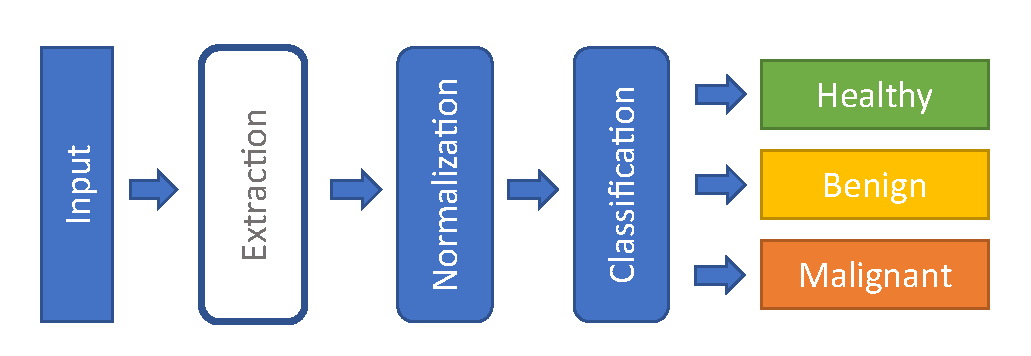
\includegraphics[width=2.5in]{content/figures/Process.pdf}
  \caption{Overall classification process. Extraction step is changed depending on the current evaluated method.}
  \label{fig:pipeline}
\end{figure}
The first method intends to classify our \ac{rcm} images using an hand-crafted feature extraction by use of the wavelets as suggested by a recent article~\cite{Halimi2017a}. The main idea is to perform characteristics extraction with Daubechies wavelets along three axes: horizontal, vertical and diagonals. Extraction of wavelets is performed by using “PyWavelet” library~\cite{lee2006pywavelets}. Then reduction of the number of parameters is achieve to avoid a data overfitting and a time-consuming computation. Extracted coefficients are reduced using Generalized Gaussian Distribution by keeping only $\alpha$ and $\beta$, respectively the scale and shape parameters of this distribution (see \Cref{eq:ggd}). To ease the readability, we will call this method “Wavelets”.\par
\begin{equation}
    f(x)= \frac{\beta}{2\alpha\Gamma(1/\beta)} \; e^{-\left(\frac{|x-\mu|}{\alpha}\right)^\beta}
    \label{eq:ggd}
\end{equation}
The second proposed method for feature extraction is performed using Haralick texture descriptors~\cite{Haralick1973} as input information for classifier. These characteristics are extracted along four axes: horizontal, vertical and two diagonals. These are statistical-based descriptors, efficient in describing pattern on texture images. Haralick features are extracted using “Mahotas” library~\cite{coelho2012mahotas}. For the sake of clarity, we will call this method “Haralick” in the remainder of this paper.\par
The last method we propose is based on \acsp{cnn}. These networks are well-suited methods for image classification, by means of extracted complex and robust feature patterns. Our work focuses on Google “InceptionV3” architecture~\cite{Szegedy2015} as it is supposed to perform well on medical images according to recent studies~\cite{Litjens2017}. Instead of training this network from scratch, we choose a Transfer Learning approach which is appropriate for a problem similar to the original database and when the amount of data is reduced. Moreover, this model is originally trained on ImageNet database~\cite{Deng2008}, provides generic image descriptors that allows to describe efficiently new images. In order to get this new representation of data, we removed the last layers devoted to classification. As our retrained network is expected to use multi-scaled input images, we added a pooling layer at the end of the remaining hidden layers in order to get features with a constant dimension independently from the input image size. Furthermore, “Max Pooling” is used instead of “Average Pooling”, as it is considered reproducible and more suitable to input image size variations. Implementation is made with help of “Keras” library~\cite{chollet2015keras}. For convenience, this method will be called “Deep Learning” in the next paragraphs.\par